%%%%%%%%%%%%%%%%%%%%%%%%%%%%%%%%%%%%%%%%%%%%%%%%%%%%%%%%%%%%%%%%%
%%%  Capstone Project Template that tries to save a few trees %%%
%%%  Edwin Blake 22 Aug 2013                                  %%%
%%%		1 Aug 2014 (revised)                          %%% 
%%%             10 Aug 2015                                   %%%
%%%  see also                                                 %%%
%%% http://ravirao.wordpress.com/2005/11/19/latex-tips-to-meet-publication-page-limits/  
%%%%%%%%%%%%%%%%%%%%%%%%%%%%%%%%%%%%%%%%%%%%%%%%%%%%%%%%%%%%%%%%%

\documentclass[11pt,a4paper]{article}
\usepackage{times}
\usepackage{fancyhdr}           % Allows better control over headers and footers
%\usepackage{layout}            % use with \layout to see the page layout for
%debugging purposes.
\usepackage[margin=2.5cm]{geometry}  %   set the margins using the
                                %   geometry package (which is much
                                %   the easiest way of doing this).
\usepackage[pdftex]{graphicx}   %   Pictures (means you have to
                                %   produce pdf output via pdflatex)
\usepackage[small,compact]{titlesec}   % Try to reduce the white space
                                % latex loves so much
\titlelabel{\thetitle. \quad}   % Reduce space around section heads
                                % and add a full stop after the number
\pagestyle{fancy}               % Invoke fancy headers

\renewcommand{\abstractname}{\vskip -5mm}  %  Change name of Abstract
                                %  to nothing and loose some of the
                                %  excessive white space
\begin{document}

\title{UAVpath:Capstone Project Report} \date{}
\author{Lethabo Neo\\Department of Computer Science\\nxxlet001@myuct.ac.za
\and Max Mkhabela\\Department of Information Systems\\mkhmax003@myuct.ac.za
\and Kenneth Baloyi\\Department of Computer Science\\blyken001@myuct.ac.za}
\cfoot{\thepage}
%%%  Set the headers via fancyhdr package
\lhead{Capstone Project Report }  % Short title for running head
\chead{}
\rhead{\thepage}   %  Fixed running head of the date
\lfoot{}

\rfoot{}
\renewcommand{\headrulewidth}{0.0pt}   % Don't want horizontal line
                                % under header.

\maketitle
\thispagestyle{plain}  % First page is plain style headings and
                       % footers (ie just the page number as footer).

\section{Approach}

\ref{ss:conclusion}.

\subsection*{Abstract}
This capstone project develops a 3D visualisation system for Unmanned Aerial Vehicle (UAV) flight trajectories, enabling users to preview, compare and analyze paths generated by flight planning algorithms. The system supports loading 3D models of structures, load trajectory data, rendering smooth paths with spline interpolation, visualizing waypoints with orientation markers, and providing a first-person view (FPV) preview. It supports multi-trajectory comparisons with metrics like path length, vertical displacement, and estimated duration. The system further allows real time waypoint editing with FPV updates and optimised rendering for large trajectories. 

\subsection{Introduction}
\label{ss:introduction}
Unmanned Aerial Vehicles (UAVs or drones) are increasingly used for photogrammetric reconstruction of terrestrial structures, such as cultural heritage sites, where high-quality images are captured to build detailed 3D models. Manual flight path planning is time-consuming and inefficient, leading to research in automated algorithms that generate optimal paths minimizing flight time and image count. This project focuses on creating a 3D visualization system for UAV flight trajectories, allowing users to preview paths, compare trajectories from different algorithms, and export mission data for real-world deployment.

This project addresses key challenges in UAV flight path planning by providing an interactive environment for loading 3D scenes (OBJ/PLY models), parsing waypoint data (positions, yaw, pitch), interpolating smooth curves, and calculating efficiency metrics. Users can edit waypoints in real time, view FPV simulations, and compare multiple trajectories side-by-side. The coordinate system uses XYZ for positions (meters) and yaw/pitch for orientations (degrees), with roll assumed level for stability.

The project adopted an Agile methodology, allowing interative development with weekly  sprints for features like trajectory parsing and FPV previews, waypoint editing, and metric calculations. Non-functional requirements emphasize performance (real-time rendering for large datasets), usability (intuitive GUI with keyboard/mouse controls), and portability (Python-based for cross-platform use).

\subsection{Requirements Captured}

1. First-Time Scene Loading and Exploration

• Actor: UAV Operator

• Trigger: The operator needs to view a 3D structure before analyzing
the flight path.

• Flow: The operator loads a 3D model into the application to display the scene for path planning. The system renders the model in the main viewport and FPV side panel from a default bird's-eye view, with axes for orientation. The operator manipulates the camera via keyboard/mouse.

• Alternative Paths: Invalid file (error message), corrupt file (termination with error), missing materials (default rendering with warning).

2. Visualizing and Understanding a Flight Path

• Actor: UAV Operator

• Trigger: The operator needs to evaluate a flight path.

• Flow: With a 3D model loaded, the operator loads a trajectory file (JSON). The system processes waypoints, renders a navigable 3D curve with orientation markers, and displays camera positions.

• Alternative Paths: Invalid trajectory (error handling).

Additional Use Cases (derived from code and project spec):

3. Comparing Multiple Trajectories

• Actor: UAV Operator

• Trigger: The operator needs to survey multiple path options to
evaluate.

• Main Success Scenario: Operator loads multiple trajectories, views them overlaid in the 3D scene with different colors, and compares metrics (length, duration, efficiency rating) in a sidebar.

4. Editing Waypoints and FPV Preview

• Actor: UAV Operator

• Main Success Scenario: Operator selects a waypoint, adjusts position/orientation via keyboard, views real-time FPV, and saves changes.

\subsection{Design Overview}
\label{ss:design-overview}

The system design is modular, with clear interfaces for independent modification. It uses a layered architecture: Data Layer (trajectory parsing, JSON handling), Rendering Layer (Open3D for 3D visualization, Trimesh for meshes), UI Layer (Tkinter GUI with threading for updates), and Logic Layer (interpolation, metrics).

Key classes include Trajectory (holds waypoints, calculates metrics), Waypoint (position, yaw, pitch), UAVVisualizationApp (main GUI), and UpdateLoopManager (handles rendering threads).

Algorithms: Spline interpolation (CubicSpline) for smooth paths; metric calculations for length, vertical displacement, turning angle, and efficiency rating (weighted formula).

Data organization: Waypoints as lists of dataclass objects; positions as NumPy arrays for efficient computations.

\begin{figure}[h!]
  \center{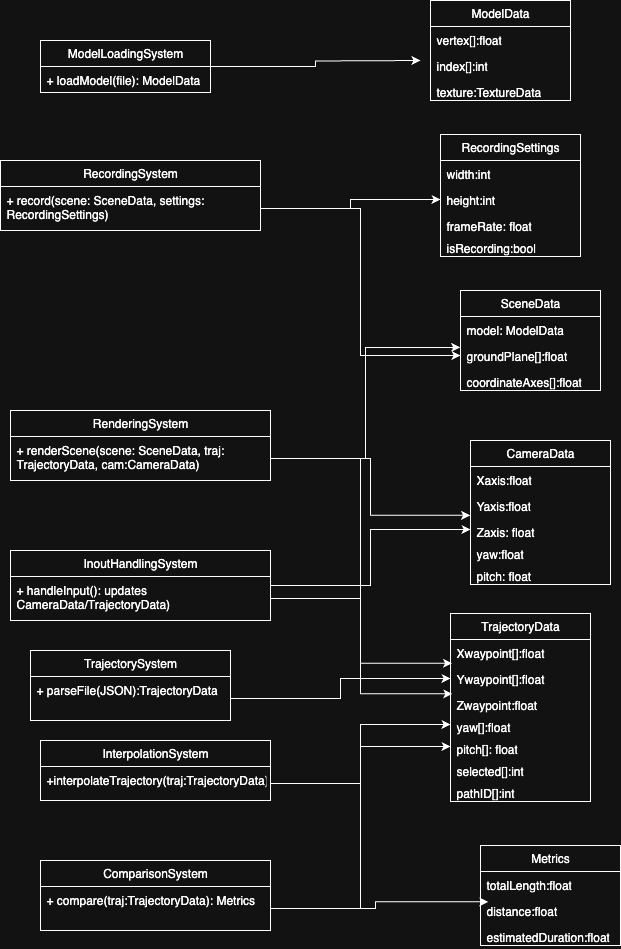
\includegraphics[scale=0.8]{analysis.png}}  % Replace with your class diagram
  \caption{Class Hierarchy Diagram.}
  \label{fig:classhierarchy}
\end{figure}

\begin{figure}[h!]
  \center{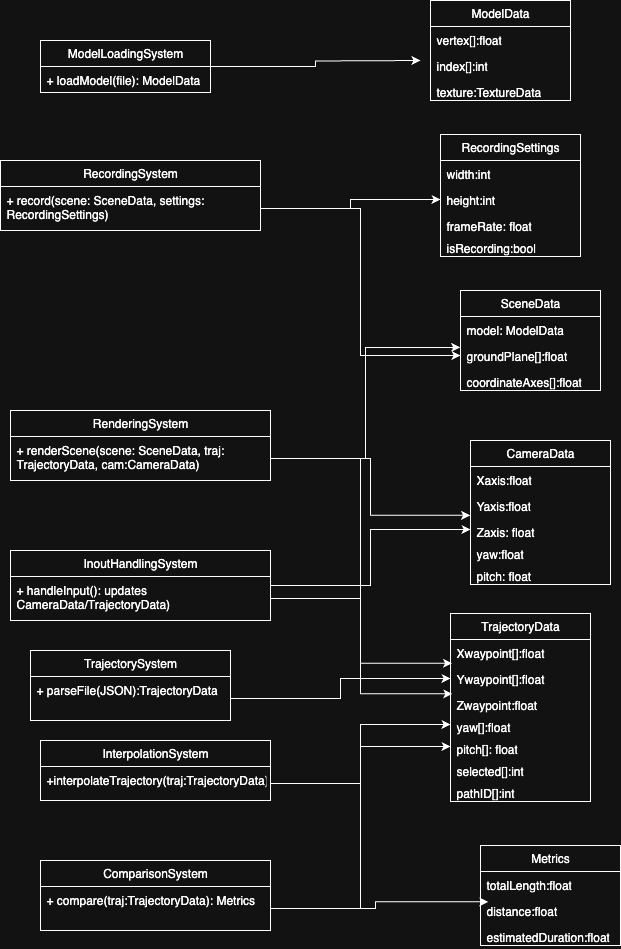
\includegraphics[scale=0.8]{analysis.png}}  % Replace with your actual diagram file
  \caption{Use Case Diagram showing key interactions.}
  \label{fig:usecase}
\end{figure}

You must present the overall architecture of the system together with
an architecture diagram. You may choose what kind of diagram best
suits your project but we would expect a layered architecture diagram
(see Figure \ref{fig:architecture}) unless there is a good reason for
some other kind of diagram. It need not be a formal UML diagram as
long as it conveys all the necessary information clearly.

You should then (in subsections) cover the algorithms and the data
organisation used and why they were considered the best. 

\subsection{Implementation}

The system was implemented in Python 3.12 using Open3D for 3D rendering, Trimesh for mesh loading, SciPy for interpolation, and Tkinter for the GUI. Data structures: NumPy arrays for positions; dataclasses for Waypoint/Trajectory.

User interface: Collapsible frames for controls; canvas for main view; label for FPV; text widget for metrics.

Significant methods: Trajectory.calculate_detailed_metrics() (computes length, angles); UAVVisualizationApp.update_trajectory_visualization() (renders paths/markers); keyboard handlers for editing.

Special techniques: Threading for non-blocking updates; Open3D's offscreen rendering for FPV images.

Libraries: numpy, scipy, open3d, trimesh, tkinter, PIL.

\begin{figure}[h!]
  \center{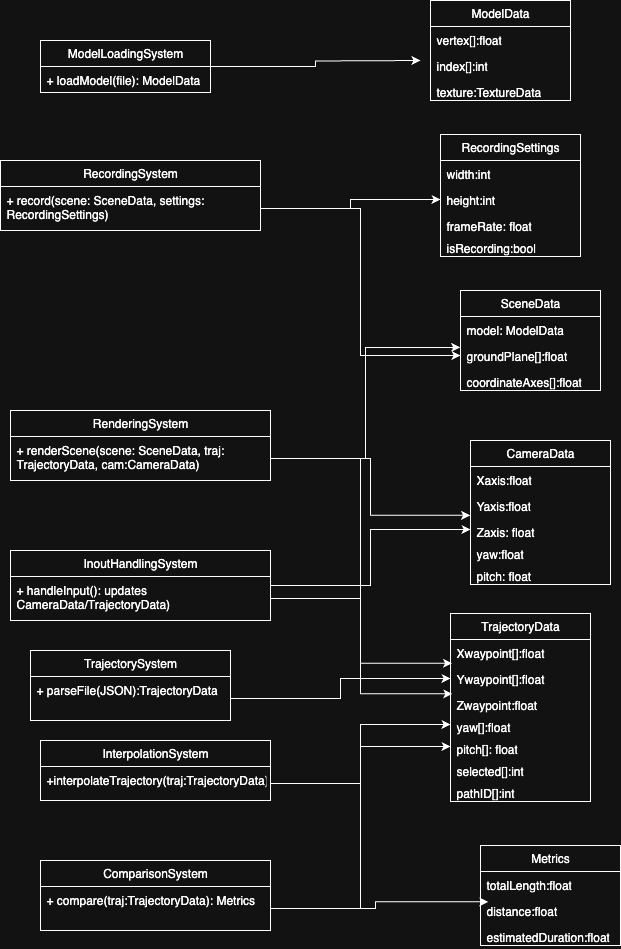
\includegraphics[scale=0.8]{analysis.png}}  % Add your app screenshot
  \caption{GUI Screenshot showing trajectory visualization.}
  \label{fig:gui}
\end{figure}

\subsection{Program Validation and Verification}
\label{ss:progr-valid-verif}

Quality Management Plan: Unit tests for parsing/interpolation; integration tests for rendering; validation via use cases; system tests for performance.

Types of testing:

\begin{table}[h!]
  \centering
\caption{Summary Testing Plan.}

\begin{tabular}[t]{|p{8cm}|p{7cm}|} \hline

  \textbf{Process} & \textbf{Technique} \\ \hline 1. Class
    Testing: Methods for waypoints/metrics & Unit tests with pytest \\ \hline 2. Integration Testing:
    GUI + Rendering & Behavioral tests with mock data \\ 
    \hline 3. Validation Testing: Meets requirements & Use-case based black box \\ 
    \hline 4. System Testing: Large models/trajectories & Stress tests for FPS/memory \\ \hline

\end{tabular}

\label{tab:test-plan}
\end{table}

Test results: [Insert your test data here, e.g., from running pytest on vis.py]

\begin{table}[h!]
  \centering
\caption{Table of Tests.}

  \begin{tabular}[t]{|p{5.5cm}|p{3cm}|p{3cm}|p{3cm}|} \hline \textbf{Data Set
    and reason} & \multicolumn{3}{c|}{\textbf{Test Cases}}\\
    \cline{2-4} & \emph{Normal} & \emph{Boundary} &
    \emph{Invalid} \\ \hline Small trajectory (10 waypoints): Basic loading & Passed & n/a & Error handled \\\hline Large mesh (1M vertices): Performance & Passed (20 FPS) & Slow (10 FPS) & Crash prevented \\\hline &&&\\ \hline
  \end{tabular}

\label{tab:tests}
\end{table}

User tests: [Describe any user feedback, e.g., "5 testers found FPV intuitive."]

The system is usable for previewing paths, with high efficiency for small datasets.

\subsection{Conclusion}
\begin{tabular}[t]{|p{8cm}|p{7cm}|} \hline

  \textbf{Process} & \textbf{Technique} \\ \hline 1. Class
    Testing: test methods and state behaviour of classes & Random,
    Partition and White-Box Tests \\ \hline 2. Integration Testing:
    test the
    interaction of sets of classes & Random and Behavioural Testing \\
    \hline 3. Validation Testing: test whether customer requirements
    are satisfied & Use-case based black box and Acceptance tests \\
    \hline 4. System Testing: test the behaviour of the system as part
    of a larger environment & Recovery, security, stress and
    performance tests \\ \hline

\end{tabular}

\label{tab:test-plan}
\end{table}
Describe all the steps taken to validate the correctness of the
program.

If you had user tests then say what you did and what the results
were. Describe why these test data were chosen (what test conditions
the data was testing).  Table \ref{tab:tests} provides an example of
the sorts of results we are looking for. The full detail of the test
runs should be appended to the report.

\begin{table}[h!]
  \centering
\caption{A table of tests. A table caption goes above the table.}

  \begin{tabular}[t]{|p{5.5cm}|p{3cm}|p{3cm}|p{3cm}|} \hline \textbf{Data Set
    and reason for its choice} & \multicolumn{3}{c|}{\textbf{Test Cases}}\\
    \cline{2-4} & \emph{Normal Functioning} & \emph{Extreme boundary cases} &
    \emph{Invalid Data (program should not crash)} \\ \hline Preliminary test
    (see Appendix 3) & Passed & n/a & Fell over \\\hline &&&\\ \hline
    &&&\\ \hline
  \end{tabular}

\label{tab:tests}
\end{table}

Follow your table of results with a discussions of them highlighting
how useful and usable your system is for its intended purpose.

\subsection{Conclusion}
\label{ss:conclusion}

Your report must have a clear conclusion where you revisit the aims
set out in the beginning and discuss how well you met them. Did you
achieve the objective of creating a well-structured, modular, and
robust system?  Please summarize the design features and test results
that show this.

\subsection{User Manual}
\label{ss:user-manual}

Your system must have a user manual. Append this to your report (make
it Appendix A) or bind it separately if it is big. If your system is
interactive and has a good user interface with context dependent help
then this can be just a cheat sheet. Discuss the level at which your
user manual is to be pitched with your client. If your system is to be
extended then you might want to include a technical API manual.

\section{Conclusion}
\label{sec:conclusion}

This document has covered the major sections needed for your
report. You will probably have each of the subsections 2.1--2.7 as
major section in the report each with its own subsections. 

A marking guide for the report will be provided later.

\appendix
\section{Code Legibility and Output}

This is not strictly part of the report but is a requirement for the
final hand-in.

\begin{itemize}
\item Each method should start wide a brief description of its
  function.

\item Use indentation to display the structure within a method.

\item Comments should be used extensively. They are best used to
  describe logical blocks of code rather than individual
  statements. Line-by-line comments have the drawbacks of not
  providing any overview and of decreasing readability.

\item Meaningful identifiers should be chosen.

\item Output should be pleasingly formatted and easy to read.
\end{itemize}

You do, of course, have the option to call in any of your
favourite packages for setting maths, graphics, computer listings,
etc.

\begin{thebibliography}{9}

\bibitem[Kopka and Daly(2004)]{KopkaDaly}
Kopka, H. and Daly, P.W.  (2004) \textit{A Guide to \LaTeXe:
Document Preparation for Beginners and Advanced Users} (4th~edn).
Addison-Wesley.

\bibitem[Lamport(1994)]{Lamport}
Lamport L. (1994) \textit{\LaTeX: A Document Preparation System}
(2nd~edn). Addison-Wesley.

\bibitem[Mittelbach and Goossens(2004)]{Companion}
Mittelbach, F. and Goossens, M., (2004) \textit{The \LaTeX\
Companion} (2nd~edn). Addison-Wesley.

\end{thebibliography}
\end{document}
